\begin{abstract}
We certify a fixed ridge predictor's regret against full-feature retraining over every continuous completion of an interval-valued table. Our main theorem gives verifiable original-row residual conditions for a uniform error bound independent of nuisance-feature scale and rank, with an asymptotically sharp leading constant and quantitative leakage stability. Full-rank constructions separate certification dimension from feature dimension, including examples requiring directions beyond the candidate. Observed-row anchors make the conditions computable, while exact row geometry and global search return valid upper bounds and feasible original-table witnesses. A finite-scale contraction and common-domain moment fallback implement the structural result. Four real-world tasks retain all model features and certify twenty rank-three instances to width $10^{-5}$. Their primary median widths improve over centered moments. Joint residual refinement additionally certifies all twenty new response-independent masks to the same precision within 76.21 seconds. For a concrete fixed-point predictor contract, pure energy certifies thirteen of fifteen stopping decisions in ten seconds, versus five for moments. Refinement certifies all fifteen within 91.68 seconds at the same objective threshold.
\end{abstract}

\section{Introduction}
Before acquiring finer training measurements, a practitioner can ask whether any legal completion would substantially improve the objective after retraining. Completion-relative regret compares a fixed candidate with each table's retrained optimum. A small uniform upper bound supports stopping acquisition; a feasible violating table rules out robust acceptance and motivates further information or a model update.

Completion-relative learning, model envelopes and repair motivate the target~\citep{zhen2024sigmod,zhu2024zorro,repair2026,vanli2014}. The retrained comparator changes with the completed table, and continuous interior worst cases can defeat endpoint enumeration. We certify arbitrary finite intervals while exploiting residual structure in the prediction task.

The central question is structural: why should a high-dimensional model admit a small certifying subspace? Feature variance describes changing inputs; regret depends on how these changes excite residuals and interact with the retrained comparator. Our original-row residual-energy conditions permit high-rank, large nuisance features on nearly fitted rows. A full-rank construction gives each uncertain column a genuine regret effect, while one learned direction supplies a small uniform error. Leading midpoint-Gram directions can miss nearly all regret even at rank $p-1$.

Residual/coercivity certification is classical~\citep{quarteroni2011,balabanov2019}. We add original-row interval conditions, a sharp uniform bound independent of nuisance scale/rank, and global certification against full retraining (Section~8). Observed anchors construct low-rank spans for four real-world tasks; the general moment verifier covers broader coarsening.
\section{Completion-Relative Ridge Regret}
Let $\cX=\prod_i[L_i,U_i]$ be a compact product of row boxes, with observed responses $y_i$, weights $w_i\geq0$, and $\lambda>0$. For a fixed candidate $\beta\in\R^p$, define
\begin{align}
 J_X(\theta)&=\sum_iw_i(x_i^\top\theta-y_i)^2+\lambda\|\theta\|^2,\\
 h_\beta(X)&=J_X(\beta)-\min_\theta J_X(\theta),\qquad
 H^*=\max_{X\in\cX}h_\beta(X).\label{eq:target}
\end{align}
The intercept, when included, is a feature and receives the same ridge penalty in our experiments. Put
\begin{align}
 M_X&=X^\top W X+\lambda I,\qquad r_X=X^\top Wy,\nonumber\\
 g_X&=M_X\beta-r_X.
\end{align}
Then $h_\beta(X)=g_X^\top M_X^{-1}g_X$. Our output is an interval $[L,U]$ with $L\leq H^*\leq U$, accompanied by a feasible original-table witness for $L$. Our fixed-point candidate uses eight-bit signed coefficients with four fractional bits, sixteen-bit inputs with ten fractional bits, and a thirty-two-bit accumulator (Appendix~\ref{app:fixed-point-v91}). The comparator is unrestricted full-feature ridge retraining.

\begin{proposition}[Endpoints can miss all regret]\label{prop:interior}
Take three observations $((t,0),0)$, $((1,0),1)$ and $((0,1),0)$ with weights $1/3$, $t\in[-A,A]$, $A>0$, and $\lambda\geq0$. For $\beta=(1/(1+A^2+3\lambda),0)$ both endpoint regrets vanish, whereas
\[
 h_\beta(t=0)=\frac{A^4}{3(1+3\lambda)(1+A^2+3\lambda)^2}>0.
\]
\end{proposition}
The endpoint and interior ridge optima follow from diagonal normal equations. At $A=1,\lambda=1/3$ the interior regret is $1/54$, with positive regularization and zero regret at both endpoints. The published SIGMOD Theorem~8.2 of \citet{zhen2024sigmod} explicitly assumes missing-value intervals $[-\infty,+\infty]$. The arXiv v2 Theorem~8.4 uses a sufficiently-wide-interval argument~\citep{zhen2024}. The 2026 repair formulation directly defines worst-completion suboptimality and searches edge repairs~\citep[Section~4.1]{repair2026}. Proposition~\ref{prop:interior} identifies the interior case that a complete certificate over finite intervals must cover.

\section{Residual Structure beyond Feature Rank}\label{sec:structure}
Put $u_X=M_X^{-1}g_X$ and $q_X(v)=2g_X^\top v-v^\top M_Xv$. For a linear subspace $S$, define the intrinsic uniform error and dimension
\begin{align}
 E(S)&=\sup_{X\in\cX}\min_{v\in S}\|u_X-v\|_{M_X}^2,\nonumber\\
 d_\varepsilon&=\min\{\dim S:E(S)\leq\varepsilon\}.\label{eq:intrinsic}
\end{align}
The identity $h_\beta(X)-\max_{v\in S}q_X(v)=\operatorname{dist}_{M_X}(u_X,S)^2$ bounds the global reduction gap by $E(S)$. Uniformity avoids the vacuous global-gap definition: one maximizing displacement alone spans a globally exact line. The energy and moment theorems bound $E$ for their physical spans. Spectral compression controls an affine span; including its offset yields linear rank at most $r+1$. Appendix~\ref{app:dimension} proves these links to classical widths~\citep{binev2011}.

We give sufficient conditions directly in the original table. Let $Q$ have orthonormal columns, $P$ be an orthonormal complement, and $\beta=Q\beta_S$. Partition rows into signal rows $\mathcal S$ and nuisance-rich rows $\mathcal N$. For every legal completion require $P^\top x_i=0$ on $\mathcal S$. Define
\begin{align*}
 A_X&=W_{\mathcal N}^{1/2}X_{\mathcal N}Q,&
 Z_X&=W_{\mathcal N}^{1/2}X_{\mathcal N}P,\\
 e_X&=W_{\mathcal N}^{1/2}(X_{\mathcal N}\beta-y_{\mathcal N}).
\end{align*}
Suppose uniformly $\|e_X\|\leq\epsilon$, $\|A_X\|_{\op}\leq a$, and
\begin{align*}
 \lambda I+X_{\mathcal S,Q}^\top W_{\mathcal S}X_{\mathcal S,Q}&\succeq\kappa I,\\
 \|\lambda\beta_S+X_{\mathcal S,Q}^\top W_{\mathcal S}
       (X_{\mathcal S}\beta-y_{\mathcal S})\|&\leq G,
\end{align*}
where $X_{\mathcal S,Q}=X_{\mathcal S}Q$ and $\kappa>0$. These conditions bound residual energy and retained signal on nuisance-rich rows, with no restriction on the size or rank of $Z_X$.

\begin{theorem}[Residual-energy certificate]\label{thm:energy}
With positive ridge, fixed nonnegative weights and a compact nonempty completion domain, put $r=\dim\operatorname{range}(Q)$, $R=(G+a\epsilon)/\kappa$ and $\eta=(\epsilon+aR)^2$. Then
\[
 E(\operatorname{range}(Q))\le\eta,\qquad d_\eta\le r.
\]
Consequently, for
\[
 V_Q=\max_{\|s\|\leq R}\max_X
 \{2g_X^\top Qs-s^\top Q^\top M_XQs\},
\]
the global enclosure is
\begin{equation}
 V_Q\leq H^*\leq V_Q+\eta.\label{eq:energy}
\end{equation}
The same enclosure holds on the containing cube $[-R,R]^r$.
\end{theorem}
\begin{proof}
At fixed $X,s$, eliminating the discarded coordinate adds
\[
 (e-As)^\top Z(\lambda I+Z^\top Z)^{-1}Z^\top(e-As)
 \le\|e-As\|^2.
\]
The retained Schur normal equation has curvature at least $\kappa$ and right-hand norm at most $G+a\epsilon$, so every full optimizer projects into the radius-$R$ ball. Apply the gain bound at that point and the pointwise error identity to obtain the uniform error. The dimension and global enclosure follow. Appendix~\ref{app:dimension} gives the full pointwise derivation and containing-box argument.
\end{proof}

Theorem~\ref{thm:energy} exploits the actual discarded curvature. A scalar-curvature residual estimate would bound its eliminated gain by $\|Z^\top(e-As)\|^2/\lambda$, which can grow without bound as discarded features are scaled. The contraction in the proof instead bounds it by $\|e-As\|^2$, uniformly in the size and rank of $Z$. Strong retained curvature also supplies the smaller radius $R$. These original-row conditions yield the dimension separation below; the leakage extension below preserves this mechanism nearby, and the general moment bound covers arbitrary tables.

\subsection{Observed Anchors and Constructive Discovery}\label{sec:anchored-energy-v84}
Let $T\in\R^{p\times p}$ be an invertible, numerically stored coordinate transformation: a parameter displacement $z$ represents the physical displacement $Tz$. Complete observations supply an aggregate quadratic anchor. Put $B=\lambda I+X_{\mathcal A}^\top W_{\mathcal A}X_{\mathcal A}$, $r_A=X_{\mathcal A}^\top W_{\mathcal A}y_{\mathcal A}$, $K=T^\top BT$, and $h=T^\top(B\beta-r_A)$. Verify $\mu I\preceq K\preceq\nu I$ for the actual $T$. For $z_0\in\operatorname{range}(Q)$ set $h_c=h-Kz_0$ and $e_c=W^{1/2}[X(\beta-Tz_0)-y]$.

\begin{corollary}[Anchored residual energy]\label{cor:anchor-energy-v84}
Partition the remaining rows into $\mathcal S,\mathcal N$ and require $X_{\mathcal S}TP=0$. Uniformly bound $\|W_{\mathcal N}^{1/2}X_{\mathcal N}TQ\|\le a$, $\|(e_c)_{\mathcal N}\|\le\epsilon$, $\|P^\top h_c\|\le d$, and
\[
 \|Q^\top h_c+(W_{\mathcal S}^{1/2}X_{\mathcal S}TQ)^\top(e_c)_{\mathcal S}\|\le G.
\]
With $c=(\nu-\mu)/2$, put
\begin{align}
 R_A&=\frac{G+a\epsilon+(c/\mu+a/(2\sqrt\mu))d+c\epsilon/(2\sqrt\mu)}{\mu},\nonumber\\
 \eta_{\rm anch}&=[\epsilon+aR_A+(d+cR_A)/\sqrt\mu]^2.\label{eq:anchor-energy-v84}
\end{align}
Then $E(\operatorname{range}(TQ))\le\eta_{\rm anch}$ and $d_{\eta_{\rm anch}}\le\dim Q$. The corresponding original retained optimum gives $V_Q\le H^*\le V_Q+\eta_{\rm anch}$; every full optimizer's retained component lies within $R_A$ of $z_0$.
\end{corollary}
The proof uses $ZD^{-1}Z^\top\preceq I$ and $\|ZD^{-1}\|\le1/(2\sqrt\mu)$ for $D=K_{PP}+Z^\top Z$. The original candidate and full retrained comparator are preserved.

Write $A=W_{\mathcal N}^{1/2}X_{\mathcal N}TQ$, $Z=W_{\mathcal N}^{1/2}X_{\mathcal N}TP$, and $e_N=(e_c)_{\mathcal N}$. Verify $\|Z\|^2\le\rho$ and $\|A^\top e_N\|\le b$. A verified radius $R\le R_A$ for both optima's retained components gives
\begin{align}
 \gamma^2&=\rho/(\mu+\rho),\nonumber\\
 E_N(R)&=\min\{(\epsilon+aR)^2,\epsilon^2+2bR+a^2R^2\},\nonumber\\
 \eta_C&=\left[\gamma\sqrt{E_N(R)}+(d+cR)/\sqrt\mu\right]^2.\label{eq:contraction-main-v89}
\end{align}
It gives $V_Q\le H^*\le V_Q+\eta_C$. The mixed moment also tightens $R$; Appendix~\ref{app:contraction-v88} gives its formula and proof. The choice $\gamma=1$, $R=R_A$ and the first residual envelope recovers~\eqref{eq:anchor-energy-v84}.

\paragraph{Common-domain adaptation.}
Let $R_c$ be the verified containing coordinate radius around the same retained reference. Aggregate discarded reference gradients and cross blocks give $G_P,C_R$ as in Theorem~\ref{thm:moment}. On this common domain use
\begin{equation}
 \eta_{\rm adapt}=\min\{\eta_C,(G_P+C_RR_c)^2/\mu\}.\label{eq:adaptive-v90}
\end{equation}
Both bounds enclose the same full-comparator problem. The single search keeps their smaller tail and pays for both verifications. Since $R_c$ is no larger than the independently centered moment radius, its sufficient tail is no larger than that moment tail. Appendix~\ref{app:contraction-v88} gives the containing-domain proof.

\paragraph{A constructive rank bound.}
Let $\theta_A=B^{-1}r_A$. Include the transformed centers and interval generators of the signal rows, and $T^{-1}(\beta-\theta_A)$, in the retained span. Taking $z_0=T^{-1}(\beta-\theta_A)$ makes $h_c=0$ and satisfies signal support. If signal row $i$ has $k_i$ unknowns, the required rank is at most $1+\sum_{i\in\mathcal S}(1+k_i)$, irrespective of nuisance rank and feature count. One signal row with one unknown therefore proposes at most three directions. Appendix~\ref{app:anchor-energy-v84} proves the construction and verifies its actual rounded implementation.

\paragraph{Support and structural rank.}
Let $J_{\mathcal S}=\{j:\exists i\in\mathcal S,\ U_{ij}>L_{ij}\}$. Under an invertible transformation $T$, exact support $X_{\mathcal S}TP=0$ for every completion implies
\[
 T^\top e_j\in\operatorname{range}(Q)\quad(j\in J_{\mathcal S}),
 \qquad r\geq |J_{\mathcal S}|.
\]
Indeed, subtract two signal rows differing only in coordinate $j$; invertibility makes the resulting generators independent. This constraint concerns uncertain signal columns. Nuisance-rich rows can have independent uncertainty in every feature. Approximate signal support is covered by the leakage extension.

\paragraph{Support leakage.} A quantitative extension allows nonzero discarded signal components, with constants converging to Theorem~\ref{thm:energy} as leakage vanishes. Appendix~\ref{app:leakage-v79} gives its original-row assumptions, radius and candidate-component correction.

\subsection{Full Rank and Many Uncertain Columns}
For $m=4^k$, take $p=m+1$, $n=2m$, weights $1/(2m)$, $\lambda=1/2$ and candidate $\beta=e_0$. Every scalar below varies independently:
\begin{align}
 x_i&=u_ie_0,&u_i&\in[3/4,5/4],& y_i&=2,\nonumber\\
 x_{m+j}&=\alpha e_0+t_je_j,&t_j&\in[\sqrt m,2\sqrt m],&y_{m+j}&=\alpha,
 \label{eq:family}
\end{align}
for $i,j=1,\ldots,m$ and dyadic $\alpha>0$. Every table has full column rank, every feature column contains a nondegenerate uncertain interval, and $\beta$ is exactly the full-feature midpoint ridge fit. Changing any nuisance $t_j$ changes regret whenever the signal gradient is nonzero. The nuisance relative interval widths and weighted feature energies stay bounded below as $m$ grows; total row energy grows with dimension.

The original and one-dimensional optima are exactly
\begin{equation}
 H^*=\frac5{4000+512\alpha^2},\qquad
 V_{e_0}=\frac1{800+512\alpha^2}.\label{eq:family_optima}
\end{equation}
Theorem~\ref{thm:energy} has $\epsilon=0$, $a=\alpha/\sqrt2$, $G=1/32$, $\kappa=25/32$ and $R=1/25$, giving error $\alpha^2/1250$, independently of $p$. At $\alpha=1/32$ this is $7.8125\times10^{-7}$, while the exact omitted regret is about $6.2453\times10^{-7}$. \begin{corollary}[Sharp leading energy constant]\label{cor:energy-sharp-v81}
Scale only the nuisance intervals in~\eqref{eq:family} by $s>0$ and put $\Delta_s=H_s^*-V_{e_0}$. For every $\alpha>0$,
\[
 \lim_{s\to\infty}\frac{\Delta_s}{\alpha^2/1250}
   =\frac{800}{800+512\alpha^2}\longrightarrow1
 \quad(\alpha\downarrow0).
\]
Thus the coefficient one in~\eqref{eq:energy} cannot be uniformly reduced over its assumption class, already at $\epsilon=0$ and retained rank one.
\end{corollary}
Schur elimination gives the limit; Appendix~\ref{app:scale-v80} supplies the exact full-rank original-row calculation.

\paragraph{Automatic direction recovery.} The uncertainty-gradient proposal defined in Appendix~\ref{app:new} recovers $e_0$ under scalar ridge-anchor preprocessing: first-order signal terms cancel, second-order terms lie in $e_0$, and nuisance generators vanish at the fitted candidate.

The endpoint-average second moment has at least $m$ eigenvalues $\ge5/4$, forcing rank-$r$ uniform ridge-whitened tails to have $\rho\ge5/2$ for $r\le m-1$. At $\alpha=1/32$, every leading midpoint-Gram PCA span of rank $1\le r\le p-1$ captures at most $9/3271682$, about 0.23\% of $H^*$. One residual-oriented direction suffices; Appendix~\ref{app:energy} proves these specific Gram-PCA and spectral comparisons.

\noindent\begin{minipage}{\columnwidth}
\begin{proposition}[Intrinsic dimension beyond one]\label{prop:intrinsic-two-v83}
For the two-active-coordinate full-rank family of Appendix~\ref{app:intrinsic-two-v83}, every line $S$ satisfies $E(S)\ge25600/1371850897$, while its active plane has error at most $17/20480000$. Hence $d_{10^{-5}}=2$.
\end{proposition}
Two legal completions have orthogonal full-optimizer displacements, giving the lower bound for every line. The energy theorem supplies the plane upper bound; the appendix gives the exact original-row proof.
\end{minipage}

\begin{figure*}[t]\centering
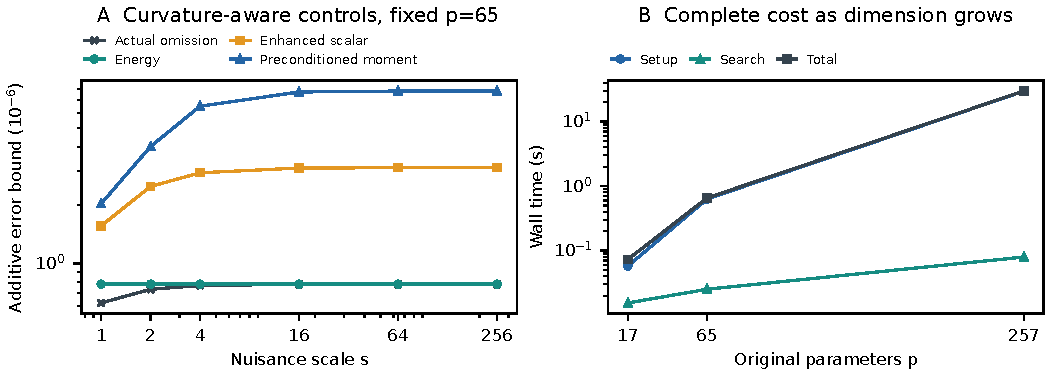
\includegraphics[width=\textwidth]{images/structure_main_v82.pdf}
\caption{The structural gain and its complete cost. (A) At fixed $p=65$, energy, enhanced scalar curvature and an actual dyadically preconditioned moment bound all remain bounded under nuisance scaling; energy has the smallest bound. These additive tails precede independent original-objective caps. (B) Single complete-pipeline timings at $\alpha=1/32$ and retained rank one. Setup includes input, anchor and method verification; their sum with search is the total. The ten-second search cap excludes setup; at $p=257$, setup is $29.74$ seconds and search $0.079$ seconds.}
\label{fig:structure-main-v82}\end{figure*}

\section{Exact Row Geometry}
For $v=\beta-\theta$, expose the comparator:
\begin{align}
 H^*&=\max_v F(v),\label{eq:dual}\\
 F(v)&=\max_{X\in\cX}\{2g_X^\top v-v^\top M_Xv\}\nonumber\\
 &=\lambda(2\beta^\top v-\|v\|^2)
   +\sum_iw_i\max_{x\in[L_i,U_i]}q_i(x;v),\nonumber\\
 q_i(x;v)&=(x^\top\beta-y_i)^2-(x^\top(\beta-v)-y_i)^2.\nonumber
\end{align}
The maxima share the same pairs $(X,v)$; positive ridge and bounded data give a bounded optimizing region.
\begin{theorem}[Row-face extremizers]\label{thm:row}
There exists a maximizer of~\eqref{eq:target} in which each row has at most one nondegenerate interval coordinate strictly between its endpoints.
\end{theorem}
For a fixed comparator, projecting a row to its two residuals gives a planar zonotope with at most $2k_i$ boundary edges. Sorting the generators and checking edge endpoints and concave scalar stationary points yields an exact oracle in $O(p+k_i\log(k_i+1))$ arithmetic operations, including center projection. The same procedure handles $a^2-cb^2$, $c>0$. Segment and point images are handled directly; original-box witnesses are reconstructed from the maximizing edge. The proof, coefficient intervals and degeneracies are in Appendix~\ref{app:method-details}.

\section{Computable Certificates in an Actual Metric}
The algorithm verifies any proposed span against full-feature retraining over the original intervals. Appendix Table~\ref{tab:tails} distinguishes three sufficient bounds. The sharp spectral theorem appears in Appendix~\ref{app:spectral-v79}; the actual-metric moment bound below supports general coarsening and the acquisition study. Real-world energy uses~\eqref{eq:contraction-main-v89}.

\subsection{Observed Rows and an Actual Dense Metric}\label{sec:anchor}
Let $\mathcal A$ contain fully observed rows. With the original weights and ridge included once, form
\begin{equation}
 G_0=\lambda I+\sum_{i\in\mathcal A}w_ix_ix_i^\top,
 \qquad r_0=\sum_{i\in\mathcal A}w_ix_iy_i.
\end{equation}
General moments use a rounded inverse-transpose midpoint-Gram Cholesky factor; energy uses the observed-anchor factor. Both round $T$ elementwise to $2^{-20}$. The anchor remains $G_0$; structural controls also use ridge-only preprocessing. We verify the actual metric
\begin{equation}
 K=T^\top G_0T,\qquad 0<\mu I\preceq K\preceq\nu I.
 \label{eq:actual_metric}
\end{equation}
The moment method retains $K$ exactly. Observed rows can improve curvature and residuals independently. The spectral theorem's exact whitening and safe rounded surrogate are detailed in the appendix.

\subsection{A Regret-Oriented Residual-Moment Tail}\label{sec:moment}
For arbitrary invertible $T$, define $\widehat M_X=T^\top M_XT$ and $\widehat g_X=T^\top g_X$. Suppose $\widehat M_X\succeq\mu I$ and $U_0\geq H^*$ is valid. For a full-column-rank retained matrix $R$, put $H=R^\top R\succeq\mu_HI$ and $\Pi=RH^{-1}R^\top$. The retained original objective is
\begin{equation}
 F_R(s)=\max_X\{2\widehat g_X^\top Rs-s^\top R^\top\widehat M_XRs\}.
\end{equation}
It uses the actual anchor matrix in~\eqref{eq:actual_metric}. We compute verified constants
\begin{align}
 G_r&\geq\sup_X\|(I-\Pi)\widehat g_X\|,\nonumber\\
 C_r&\geq\sup_X\|(I-\Pi)\widehat M_XR\|_{\op},\qquad
 R_s=\sqrt{U_0/(\mu\mu_H)}.\nonumber
\end{align}
\begin{theorem}[Residual-moment certificate]\label{thm:moment}
For $\mathcal B=[-R_s,R_s]^r$, let $V_r=\max_{s\in\mathcal B}F_R(s)$. The uniform original-coordinate error satisfies $E(\operatorname{range}(TR))\le\eta_r$ and $d_{\eta_r}\le r$. Consequently,
\begin{equation}
 V_r\leq H^*\leq V_r+\eta_r,\qquad
 \eta_r=\frac{(G_r+C_rR_s)^2}{\mu}.\label{eq:moment_tail}
\end{equation}
A retained search interval $[f,U_R]$ therefore gives the original interval $[f,U_R+\eta_r]$, which can be tightened by any feasible full-model witness and by $U_0$.
\end{theorem}
Schur elimination bounds the discarded gain by $\|(I-\Pi)(\widehat g_X-\widehat M_XRs)\|^2/\mu$; coercivity places the full optimizer's projection inside $\mathcal B$. Appendix~\ref{app:new} details the actual-metric calculation.

Aggregate coordinate ranges are summed across rows before taking norms, preserving cancellation near a midpoint optimum. Verified midpoint cross blocks and original row-interval perturbations supply $C_r$. Uncertainty-gradient generators propose $R$; its actual Gram/projector and every tail constant determine the guarantee. Appendix~\ref{app:new} gives their formulas.

\section{Complete Search and Complexity}
The outer objective is a maximum of concave quadratics, so direct concavity is unavailable. Its special curvature still gives a complete certificate.

For the following statement let $\mathcal F(s)=\max_X q_X(s)$ denote a search envelope, with each $q_X$ a concave quadratic; this includes $F$ and $F_R$.

\begin{theorem}[Curvature interpolation]\label{thm:interp}
Suppose the negative quadratic coefficient in coordinate $j$ is uniformly at most $H_j$. For any parameter box $B=[l,u]$,
\begin{equation}
 \sup_{s\in B}\mathcal F(s)\leq
 \max_{q\in\mathrm{vert}(B)}\mathcal F(q)
      +\frac14\sum_jH_j(u_j-l_j)^2.\label{eq:interpolation}
\end{equation}
The same statement holds with the actual nonorthogonal metric $H$ and the corresponding curvature diagonals.
\end{theorem}
The proof is in Appendix~\ref{app:method-details}.


Best-first branch and bound bisects the curvature-weighted widest side and retrains row witnesses in all features. The largest surviving leaf upper remains valid at a time cap. Outward arithmetic encloses every query. A center-gradient bound supports full-dimensional controls without root-corner enumeration.

For a root box of radius $R_0$ and exact row queries, a uniform grid with side at most $2\sqrt{\delta/\sum_jH_j}$ has global search error at most $\delta$. It uses at most
\begin{equation}
 \left[1+\left\lceil R_0\sqrt{\frac{\sum_jH_j}{\delta}}\right\rceil\right]^r
\end{equation}
grid points. The exponent is the retained model dimension $r$. Dense anchor and metric setup require $O(np^2+p^3)$ arithmetic; each attempted full-model witness fit has the same order. Proposal and tail costs are listed in Appendix~\ref{app:cost}. The total error adds its verified tail (Appendix Table~\ref{tab:tails}). Exact low rank is the zero-tail case.


\begin{proposition}[Validity and rank-adaptive completeness]\label{prop:complete-v91}
For any fixed retained rank and verified tail, every returned interval contains $H^*$. If rank enrichment reaches $p$, queries can be enclosed to arbitrary accuracy, and search time is unrestricted, then every precision $\delta>0$ is attainable with a finite original-table certificate.
\end{proposition}
At full rank the tail vanishes; a finite grid and query precision $\delta/4$ give the claimed width and a feasible original-table lower (Appendix~\ref{app:complete-v91}).

\paragraph{Refining the original domain.}
When a sufficient tail remains above the requested precision, a fixed reference $\vartheta$ gives the joint bound
\[
h_\beta(X)\le J_X(\beta)-J_X(\vartheta)+\mu^{-1}\|T^\top(M_X\vartheta-r_X)\|^2.
\]
Its degree-four cell polynomial preserves the objective--residual dependence. A moment relaxation with independently validated dyadic duals bounds each completion box; covering subdivision refines the global interval. This supplies a precision fallback with the same full retrained comparator (Appendix~\ref{app:joint-refinement-v92}).

\subsection{Rank Selection and Error Allocation}
Our selector searches specified proposals at ranks 1,2,3 for a verified tail at most $2.5\times10^{-6}$. It returns a verified sufficient rank when available. Otherwise, the span with the smallest verified tail supplies the first-stage interval, and joint residual refinement continues toward the requested total precision.

Algorithm~\ref{alg:certificate} in Appendix~\ref{app:joint-refinement-v92} gives the full procedure.

The total error is search plus tail, with a verified anchor error for identity-metric surrogates; the actual-metric moment method has zero anchor error. The complete interval determines precision, and its endpoints remain valid at every checkpoint. The decision is STOP if $U\leq\tau$, violating if $L>\tau$, and unresolved otherwise. Width $U-L$ measures numerical precision; $\tau$ is the model-retention tolerance. If $U\le\tau$, every full retrained optimum satisfies
\[
 |z^\top(\beta-\theta_X^*)|\le\sqrt{\tau z^\top G_0^{-1}z}
\]
for any feature vector $z$, using $M_X\succeq G_0\succ0$. This bounds prediction deviation from full retraining (Appendix~\ref{app:extensions}).



\begin{figure*}[t]\centering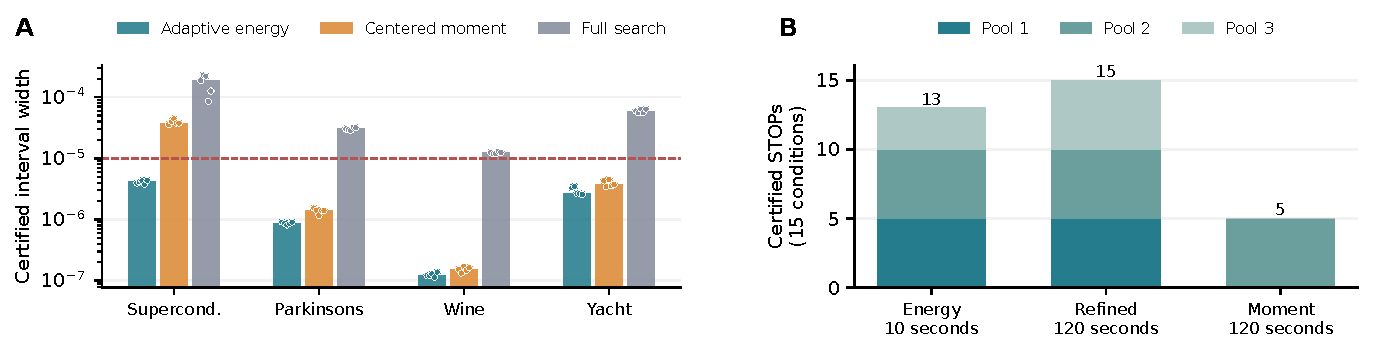
\includegraphics[width=.97\textwidth]{images/public_energy_v84.pdf}
\caption{Residual structure connects precision to acquisition decisions. A: four tasks with five masks each, all features retained; points are masks and bars are median widths under ten-second complete budgets. B: the fixed 2\% rule on fifteen conditions in three disjoint pools. Energy certifies thirteen STOPs by ten seconds. Refinement certifies all fifteen by 120 seconds, versus five for moments at the same deadline, avoiding 330 additional cells under the fixed thirty-three-cell policy.}\label{fig:public-energy-v84}\end{figure*}


\section{Experiments}\label{sec:experiments}
We test residual structure, full-feature certification and decision value. Timed pairs use one pinned i7-13800H logical CPU and single-thread libraries, reserving two performance cores. Additional queues report their own conditions. Deterministic enclosures cover masks on fixed record pools. Code and protocols: arXiv source archive, \texttt{anc/README.md}; \url{https://github.com/Peida-Lee/certifying-retraining-regret}.

\subsection{The Structural Separation in Computation}
The family~\eqref{eq:family} crosses $m=16,64,256$ with $\alpha=0,1/64,1/32,1/16$. Both methods share the learned rank-one direction, full comparator, ten-second search cap and $10^{-6}$ target. Energy verifies the conditions and meets all twelve targets; moment meets the three zero-coupling targets, reaches six tail floors and exhausts three caps. At $p=65,\alpha=1/32$, widths are $0.657\times10^{-6}$ versus $57.1\times10^{-6}$. Complete energy costs are $0.073,0.655,29.82$ seconds at $p=17,65,257$ (Figure~\ref{fig:structure-main-v82}B). The largest case spends $29.74$ seconds in setup and $0.079$ in search (Appendix~\ref{app:cost}).

\paragraph{Curvature-aware controls at fixed dimension.}
Fix $p=65$, the candidate, direction and signal intervals, and scale nuisance features by $s\in\{1,2,4,16,64,256\}$. Energy stays $\alpha^2/1250$. An enhanced scalar-curvature bound is $2\alpha^2s^2/[625(1+s^2)]$; a verified preconditioner $T_s=\operatorname{diag}(1,s^{-1}I)$ also keeps moments bounded. Figure~\ref{fig:structure-main-v82}A compares these stronger controls with exact omitted regret. Energy is sharper across this diagonal family (Appendix~\ref{app:scale-v80}).

\subsection{Automatic Multidimensional Structure}
Eighteen two/three-active-coordinate conditions test learned directions. In the unperturbed cases, candidate-line errors exceed $2\times10^{-4}$ while learned energy tails are below $8.34\times10^{-7}$. A verified sparse-block elimination completes the full residual/leakage grid to width $10^{-5}$ in 0.06--0.13 seconds per condition. Appendix~\ref{app:multirank-v82} reports the structural first-stage ablation and all eighteen exact block audits.

Nonzero-residual and leakage series, including six automatic rank-one cases, appear in Appendices~\ref{app:epsilon}, \ref{app:leakage-v79} and \ref{app:auto-energy-v80}.

\subsection{Real-World Experiments}
We evaluate Superconductivity, Parkinsons Telemonitoring, Wine Quality and Yacht Hydrodynamics~\citep{uci_super,uci_parkinsons,uci_wine,uci_yacht}. Every model retains all supplied predictor columns and its intercept. Recorded outcomes use the specified affine normalization and $2^{-10}$ quantization. Each instance has one signal-row unknown and sixteen nuisance rows with two unknowns each, giving 33 uncertain cells across multiple features. The candidate is midpoint ridge rounded to four fractional binary bits; the comparator retrains in all original features. The signal row has maximum pilot residual; sixteen nuisance rows are sampled from the 32 smallest residual-interval scores after three fixed passes. Five masks per task use the constructive rank-three span.

Adaptive energy~\eqref{eq:adaptive-v90} gives the smallest median width among A, M and full search on all four datasets (Figure~\ref{fig:public-energy-v84}, Table~\ref{tab:public-energy-v84}). The median paired width reductions against independently centered moments are 89.7\%, 38.4\%, 20.3\%, 25.3\%, respectively. All twenty adaptive intervals meet $10^{-5}$ precision within ten-second complete budgets. Appendix~\ref{app:public-energy-v84} reports the tail and search contributions to this total precision. The comparison uses identical row boxes, candidates, retained spans, feasible midpoint witnesses and coarse caps. Preprocessing, bound verification, search and full-feature witness fits all enter the budget.

The refined contraction links the structural theorem to these gains: verified discarded row energy reduces the contraction factor, and mixed residual moments tighten the retained radius and residual envelope. Independent rational audits reconstruct twenty primary receipts and feasible original-table witnesses, including a complete search tree for each dataset. Appendix~\ref{app:public-energy-v84} gives the full parameters, paired runs and cost breakdown.
\begin{table*}[t]\centering\small\setlength{\tabcolsep}{4pt}
\caption{Four real-world tasks, all features and five masks retained. All regret quantities use $10^{-6}$ normalized-objective units. $h_c$ is midpoint regret; the increment column bounds the median of $H^*-h_c$. Widths are marginal medians; gain is the median paired width reduction against M. A is adaptive energy and M independently centered moments. All methods have ten-second complete budgets.}
\label{tab:public-energy-v84}
\begin{tabular}{lrrrrrrr}\toprule Data&$p$&$h_c$&Increment bounds&A width&M width&Full width&Gain\\\midrule
Supercond. & 82 & 1664.298 & [23.232, 27.351] & 4.119 & 37.438 & 186.00 & 89.7\%\\
Parkinsons & 20 & 817.937 & [10.773, 11.677] & 0.862 & 1.403 & 30.10 & 38.4\%\\
Wine Quality & 12 & 424.515 & [2.323, 2.461] & 0.122 & 0.153 & 12.49 & 20.3\%\\
Yacht & 7 & 744.339 & [17.220, 19.789] & 2.669 & 3.723 & 58.99 & 25.3\%\\
\bottomrule\end{tabular}\end{table*}

Matched controls vary nuisance-row sampling and candidate precision on the same boxes. With a common 600-second cap, refinement certifies all twenty-four matched conditions to width $10^{-5}$ and centered moments certify fifteen. Refinement's measured algorithm costs are at most 459.69 seconds from the stored inputs. Appendix~\ref{app:precision-controls} separates the ten-second first-stage ablation from refinement; Table~\ref{tab:public-energy-v84} links midpoint cost, uncertainty increment and precision.

\paragraph{Response-independent masks and precision refinement.}
We evaluate five further masks per task, with all seventeen row indices sampled independently of responses and residuals. The reference, branching and solver rules are fixed before these runs. Our complete algorithm reaches $10^{-5}$ width in all twenty instances: eight complete by 10 seconds, sixteen by 60 seconds and all twenty by 120 seconds. The longest complete run is 76.21 seconds; centered moments reach the target in five instances under the common 600-second cap. Table~\ref{tab:independent-v91} compares the final full-comparator certificates and success counts. Appendix~\ref{app:core-decisions-v91} gives the structural-stage ablation and every mask; Appendix~\ref{app:joint-refinement-v92} gives the polynomial bound, validated moment dual and complete timing protocol.
\begin{table}[t]\centering\small\setlength{\tabcolsep}{2.5pt}
\caption{Five new response-independent masks per task. Median widths use $10^{-6}$ units. Our complete algorithm combines structural certification and joint refinement; M is centered moments. Time includes all algorithm stages. Success counts use the common $10^{-5}$ target and 600-second cap.}\label{tab:independent-v91}
\begin{tabular}{lrrrrrr}\toprule Data&Ours width&M width&Ours (s)&Ours&M\\\midrule
Supercond. & 3.174 & 254.4 & 65.55 & 5/5 & 0/5\\
Parkinsons & 0.1055 & 57.95 & 52.29 & 5/5 & 0/5\\
Wine Quality & 6.321 & 7.278 & 6.03 & 5/5 & 5/5\\
Yacht & 0.001748 & 25.39 & 9.92 & 5/5 & 0/5\\
\bottomrule\end{tabular}\end{table}

\begin{table}[t]\centering\small\setlength{\tabcolsep}{3pt}
\caption{All twenty identical primary instances. Entries are median width ($10^{-6}$) / median complete seconds across five masks. A/M use outward enclosures; SCIP uses its numerical dual with $10^{-10}$ search tolerance and a nominal ten-second cap. Actual costs include indivisible-call overruns.}
\label{tab:external-main-v90}
\begin{tabular}{lrrr}\toprule Data&A&M&SCIP\\\midrule
Supercond. & 4.119 / 6.82 & 37.44 / 6.29 & 106.6 / 9.96\\
Parkinsons & 0.8616 / 4.06 & 1.403 / 4.16 & 0.7925 / 9.98\\
Wine Quality & 0.1222 / 4.60 & 0.1532 / 4.31 & 0.2836 / 9.95\\
Yacht & 2.669 / 5.29 & 3.723 / 5.12 & 0.002423 / 9.79\\
\bottomrule\end{tabular}\end{table}

The SCIP comparison covers all twenty primary masks. ZORRO refines valid model envelopes throughout its complete ten-second budget, retaining each parent's bound until child evidence is complete. Table~\ref{tab:zorro-refined-v91} and Figure~\ref{fig:zorro-time-v91} give its widths, costs and anytime trajectories on the four first masks.


\paragraph{Additional coarsening and directions.}
All sixty full-feature conditions in Diabetes, Concrete and Superconductivity~\citep{efron2004,sklearn,uci_concrete,uci_super} reach $3\times10^{-6}$ width, with independent exact replay of every certificate. Complete costs are at most 156.76 seconds (Appendix~\ref{app:general-public}). Eighteen further masks compare rank-three gradient/POD/greedy. Gradient is narrower in 16/18 and 17/18 metric-matched pairs (Table~\ref{tab:metric-v79}); twelve further SCIP controls and their objective identity audit are in Appendix~\ref{app:scip-followup}.

\subsection{Core Energy and Measurement Decisions}\label{sec:core-decisions-v91}
We freeze three mutually disjoint 1024-record Superconductivity evaluation pools, excluding the named development and scaling pools, and five masks per pool before running their solvers. One development predictor with the fixed-point contract is stored and shared across all fifteen tables. The coarsening uses the primary signal/nuisance rule. The predeclared criterion allows uncertainty to add at most 2\% to the nominal midpoint regret:
\begin{equation}
 H^*-h_\beta(X_c)\le0.02h_\beta(X_c).\label{eq:core-decision-v91}
\end{equation}
The midpoint uses only the available intervals and responses. Its verified lower endpoint defines a safe STOP threshold; its upper defines a violation threshold. Thus the rule is fixed independently of the searched worst-regret interval. Each method has ten complete seconds. The fixed acquisition policy reveals the thirty-three uncertain cells unless STOP is certified.

Pure contraction energy and adaptive energy each certify 13/15 STOPs, compared with 5/15 for centered moments and 0/15 for the common cap, SCIP and fully refined ZORRO. Energy's pool counts are $(5,5,3)$ and moment's are $(0,5,0)$. Summed across the fifteen audit instances, the policy avoids 429 cells for energy and 165 for moment, an additional 264 cells at ten seconds. Energy's median first-STOP time among its thirteen successes is 3.10 seconds. The pure and adaptive decisions coincide, identifying the structural energy bound's contribution. All ninety method-condition records and the predeclared 1\%/5\% sensitivity rules are in Appendix~\ref{app:core-decisions-v91}. A separate general-moment acquisition study appears in Appendix~\ref{app:calibration-v81}.

Joint residual refinement on the same stored instances certifies all fifteen STOP decisions within 91.68 seconds, avoiding all 495 cells under the fixed policy (Table~\ref{tab:decisions-refined-v92}). At the common 120-second checkpoint, moments certify five STOPs and refinement certifies fifteen, avoiding 330 additional cells (Figure~\ref{fig:public-energy-v84}B). The original 2\% threshold and candidate remain fixed.


\paragraph{Verification.}
Independent rational audits check original-row queries, representative complete trees and feasible table witnesses. The input-space baseline and every timing boundary are specified in Appendix~\ref{app:input} and Table~\ref{tab:protocol-v80}.

\section{Related Work and Scope}
Table~\ref{tab:closest-main-v81} summarizes the closest optimization and certification guarantees. ZORRO~\citep[Theorem 4.2]{zhu2024zorro} encloses all exact ridge optima under training-feature/label uncertainty. Its model/data zonotope can be converted to a regret upper through $h_\beta(X)=g_X^\top(\beta-\theta_X^*)$. Our direct objective bounds add an original-table lower witness and a verified residual-structure compression error; Table~\ref{tab:zorro-v90} measures the explicit model-envelope conversion. MinPrep studies cleaning necessity~\citep{minprep2026}; dataset multiplicity analyzes predictions under possible training datasets~\citep{meyer2023}. Poisoning certificates enclose perturbed training trajectories~\citep{sosnin2025,lorenz2025mibp}; interval least-squares PPS encloses solution coordinates~\citep{shary2021}. Classical widths~\citep{binev2011} and task-oriented/sketched approximation~\citep{chen2025coupled,patil2024sketched} give complementary dimension notions.
